\documentclass[tikz,border=10pt]{standalone}
\usepackage{tikz}

\begin{document}
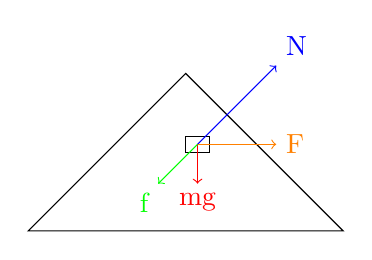
\begin{tikzpicture}

% Draw inclined plane
\draw (0,0) -- (4,0) -- (2,2) -- cycle;

% Draw block
\draw (2,1.2) rectangle (2.3,1);

% Draw forces
\draw[->,red] (2.15, 1.1) -- (2.15, 0.6) node[pos=1, below]{mg}; % gravity
\draw[->,blue] (2.15, 1.1) -- (3.15, 2.1) node[pos=1, above right]{N}; % normal
\draw[->,green] (2.15, 1.1) -- (1.65, 0.6) node[pos=1, below left]{f}; % friction
\draw[->,orange] (2.15, 1.1) -- (3.15, 1.1) node[pos=1, right]{F}; % applied force

\end{tikzpicture}
\end{document}